\documentclass[aspectratio=169, 14pt]{beamer}

\makeatletter
\def\input@path{{usyd-beamer-theme/}}
\makeatother

\usepackage{amsmath}
\usepackage{fontspec}

\defaultfontfeatures{Extension = .otf}% adds .otf to end of path when font loaded without ext parameter e.g. \newfontfamily{\FA}{FontAwesome} > \newfontfamily{\FA}{FontAwesome.otf}
\usepackage{fontawesome}

\title{\large An automated approach to crystal detection using machine learning techniques}
\date{\today}
\author[Malcolm]{Malcolm Ramsay \\ \faTwitter~@malramsay64 \\ \faGithub~malramsay64}

\usetheme{usyd}
% To use the logobar theme use the line below instead
% \usetheme[logobar]{usyd}

\titlegraphic{config_crop.png}
\titlegraphicbackground{usydred}

\graphicspath{{usyd-beamer-theme/}{figures/}}

\begin{document}

\begin{frame}
  {\fontsize{12}{14}\selectfont
  \titlepage{}
}
\end{frame}

\begin{frame}{Outline}

  \begin{itemize}
    \item Machine Learning
      \begin{itemize}
        \item What is it?
        \item Where is it useful?
        \item How can I use it?
      \end{itemize}
    \item Automated Crystal Detection
      \begin{itemize}
        \item Clustering
      \end{itemize}
  \end{itemize}
\end{frame}

\begin{frame}{Follow Along}
  \begin{center}
    \LARGE
    \url{demo.malramsay.com}
  \end{center}

  \begin{itemize}
    \item Shift + Enter to run code
    \item Run all cells from the top
  \end{itemize}

  All code and more available at \\
  \url{github.com/malramsay64/MLCrystals}

\end{frame}

\section{Machine Learning}
\begin{frame}{What is Machine Learning?}

  \begin{itemize}
    \item Technique for drawing a line
    \item Complicated methods draw complicated lines
  \end{itemize}

  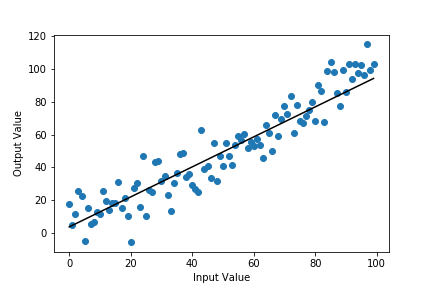
\includegraphics[width=0.5\textwidth]{drawing_lines_regression.png}
  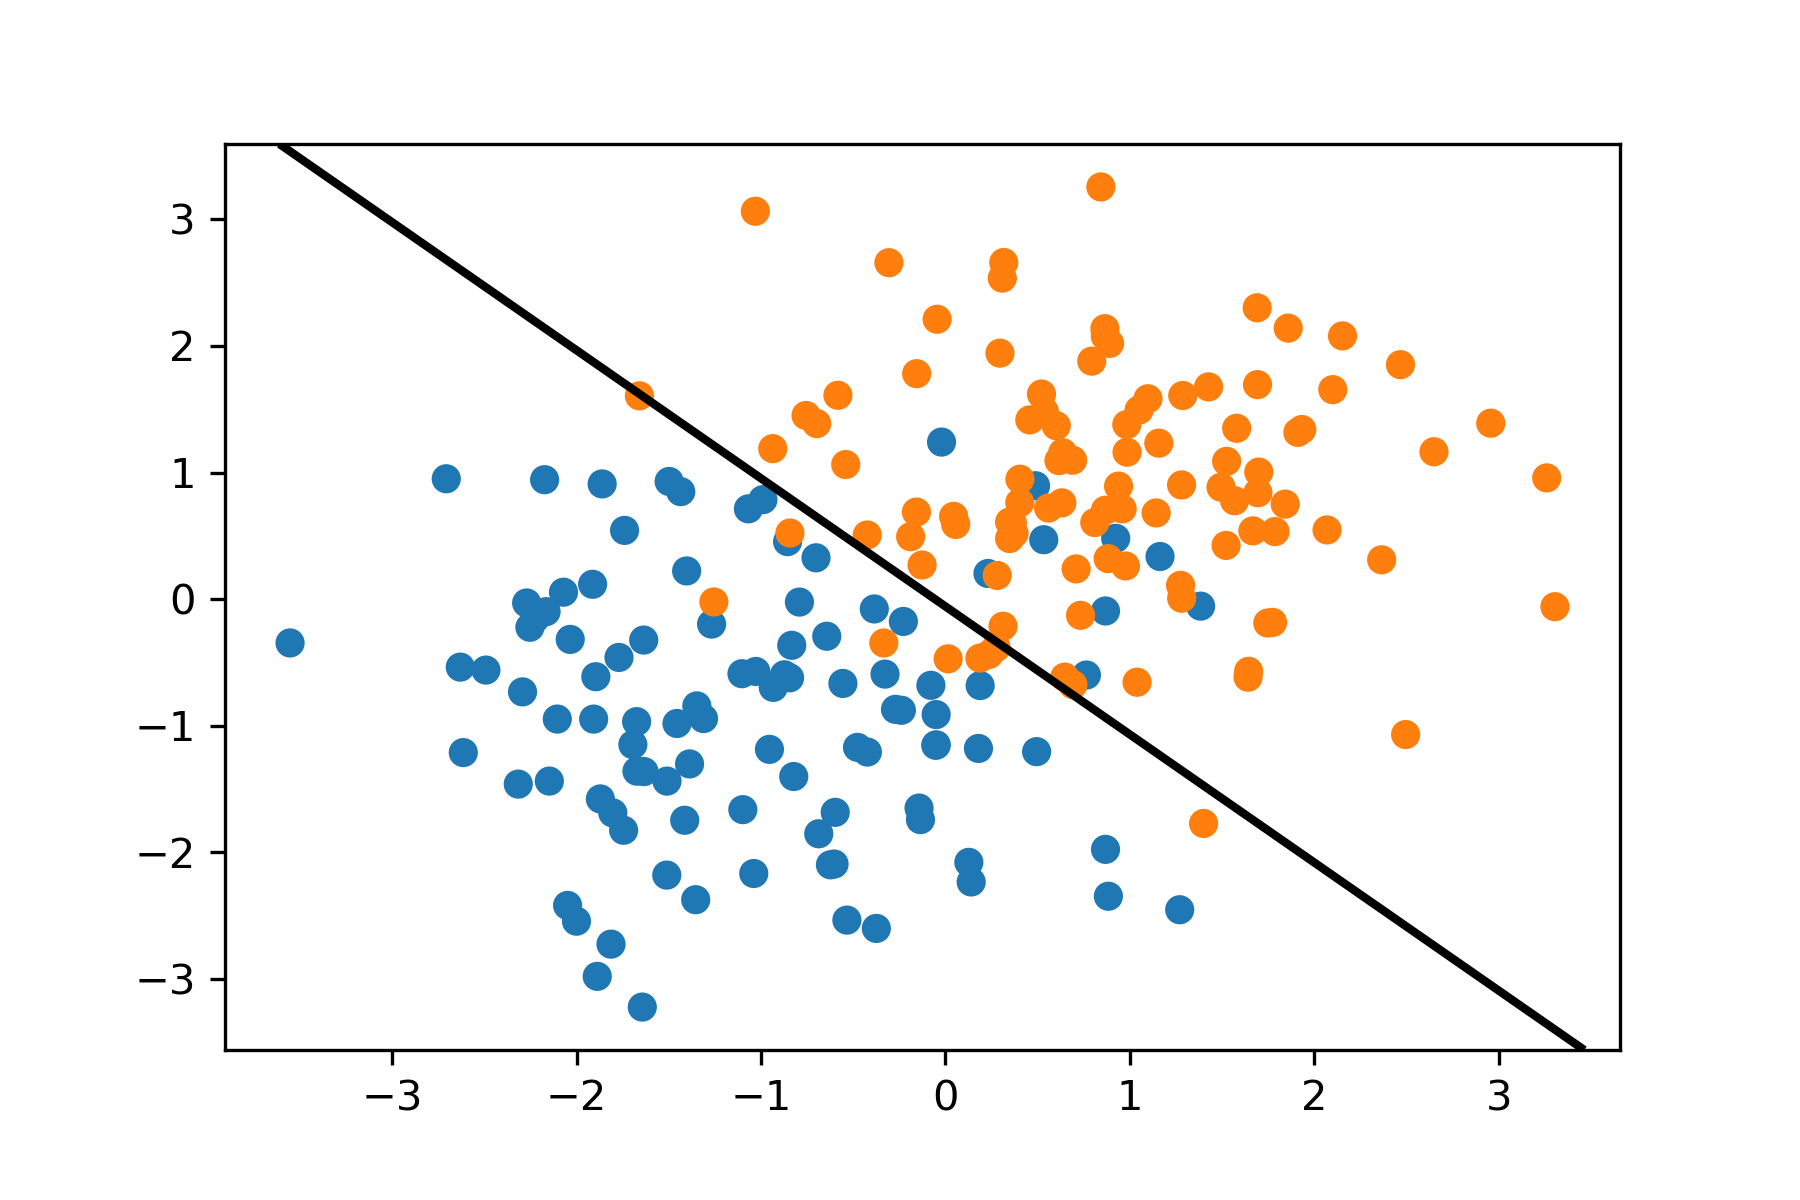
\includegraphics[width=0.5\textwidth]{drawing_lines_classification.png}

\end{frame}

\begin{frame}{Where is Machine Learning Useful}

  \begin{itemize}
    \item Classification into known groups
    \item Datasets with high dimensionality
    \item Hard to (computationally) define tasks
  \end{itemize}

\end{frame}

\begin{frame}{How to get started}

  \begin{itemize}
    \item this talk
    \item \url{kaggle.com/learn}
    \item \href{http://scikit-learn.org/stable/index.html}{scikit-learn}
  \end{itemize}

\end{frame}


\begin{frame}{Machine Learning for Classification}

  \begin{itemize}
    \item Labelled dataset, known class of each datapoint
    \item Break into training (80\%) and test (20\%) datasets
    \item Develop model on training dataset
    \item Score on test dataset
  \end{itemize}

\end{frame}

\begin{frame}{Trimer Model}

  \begin{columns}
    \begin{column}{0.4\textwidth}
      \begin{itemize}
        \item 2D rigid molecules
        \item Molecular Dynamics simulations
      \end{itemize}
    \end{column}
    \begin{column}{0.6\textwidth}
      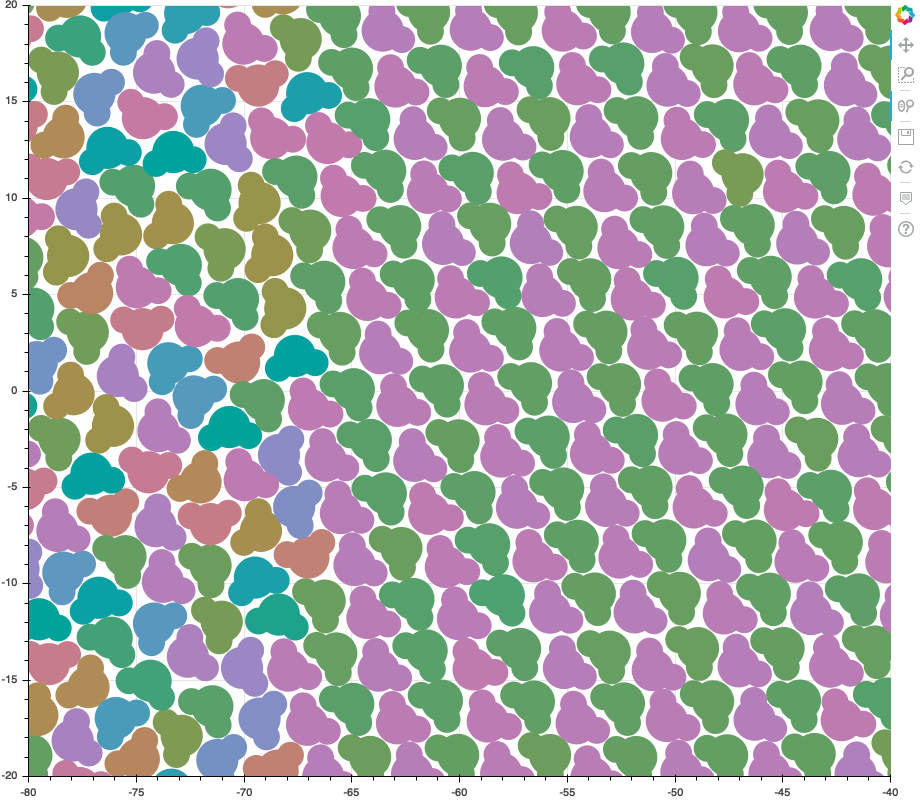
\includegraphics[width=\textwidth]{Trimer_snapshot.png}
    \end{column}
  \end{columns}
\end{frame}

\begin{frame}{Feature Identification}

  \begin{itemize}
    \item Most important part of machine learning
    \item What distinguishes the liquid from the crystal
    \item Domain expertise is important
  \end{itemize}

\end{frame}


\begin{frame}{Features in Trimer Model}

  \begin{columns}
    \begin{column}{0.5\textwidth}
      \begin{itemize}
        \item Relative orientation of nearest neighbours
        \item Invariant of crystal orientation
      \end{itemize}
    \end{column}
    \begin{column}{0.5\textwidth}
      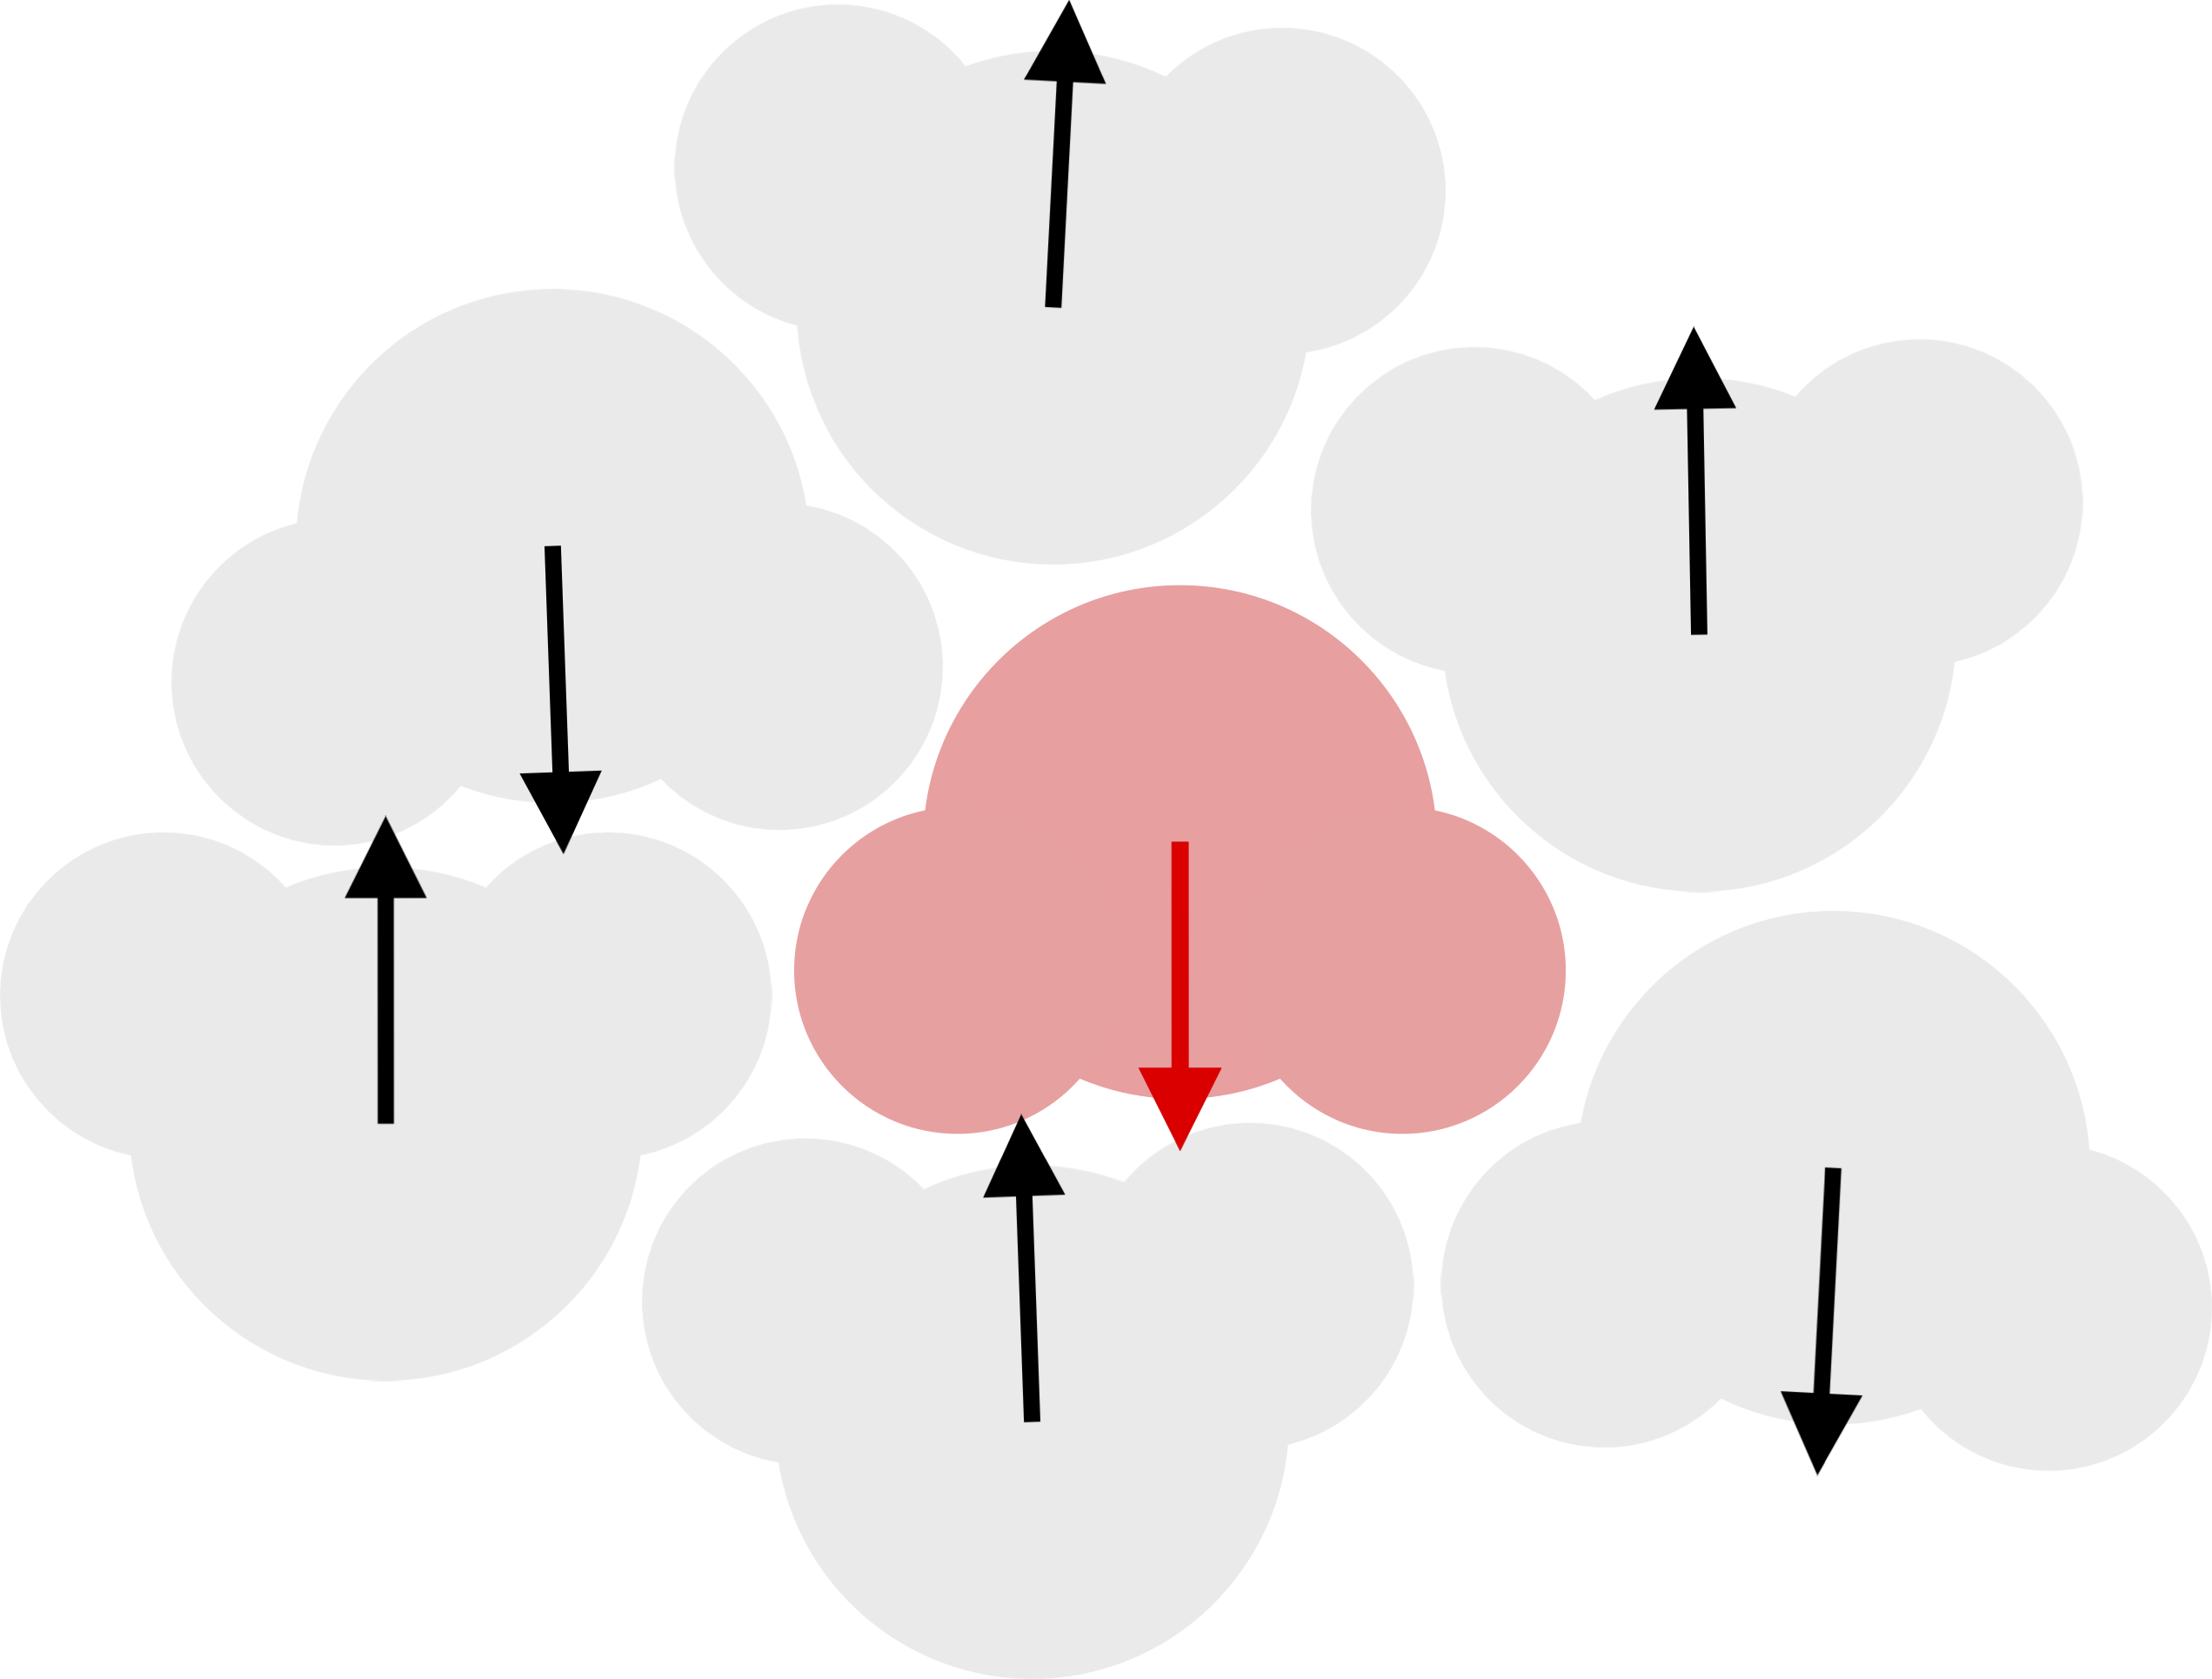
\includegraphics[width=\textwidth]{orientations.png}
    \end{column}
  \end{columns}
\end{frame}


\begin{frame}{Training and Using a Model}

  \begin{itemize}
    \item Training is the time intensive step
    \item A trained model is simple to store and use with new data
    \item No different to any other order parameter
    \item Best practice is to make dataset and code available to recreate model
  \end{itemize}

\end{frame}

\section{Clustering}
\begin{frame}{Clustering}

  \begin{itemize}
    \item How do I label 1000s of molecules?
    \item How do I know what structure is important?
    \item Which structures keep appearing?
  \end{itemize}

\end{frame}

\begin{frame}{Clustering Code}

  \begin{center}
    \includegraphics[width=0.8\textwidth]{clustering_code}
  \end{center}

\end{frame}

\begin{frame}{Clustering Trimer Model}
  \begin{columns}
    \begin{column}{0.33\textwidth}
      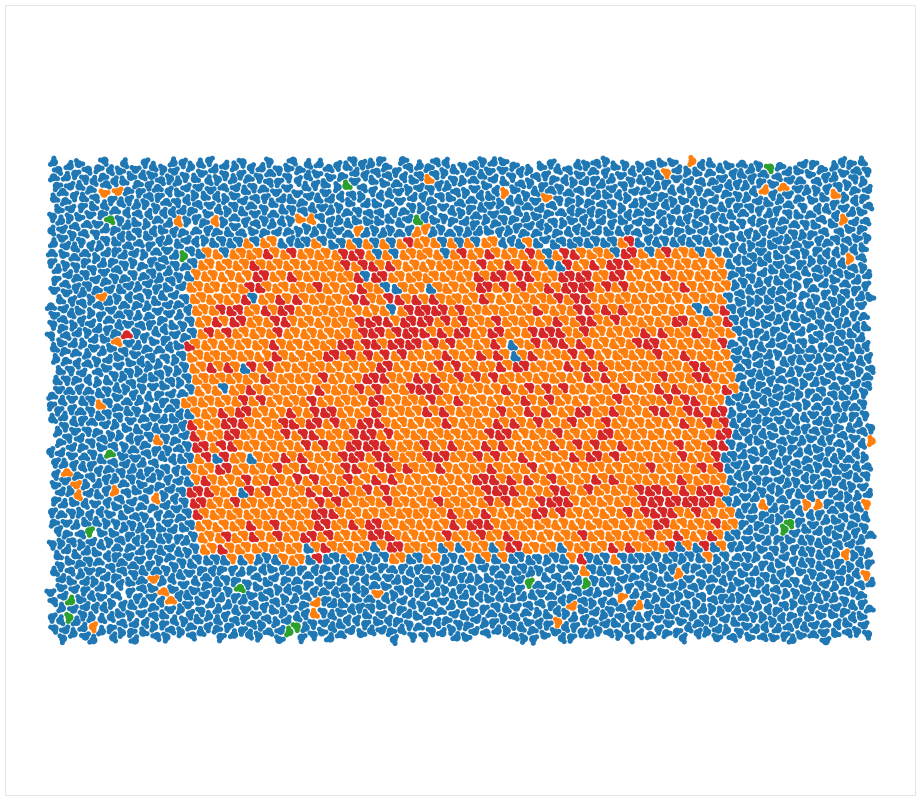
\includegraphics[width=\textwidth]{clustering_results_p2.png}
    \end{column}
    \begin{column}{0.33\textwidth}
      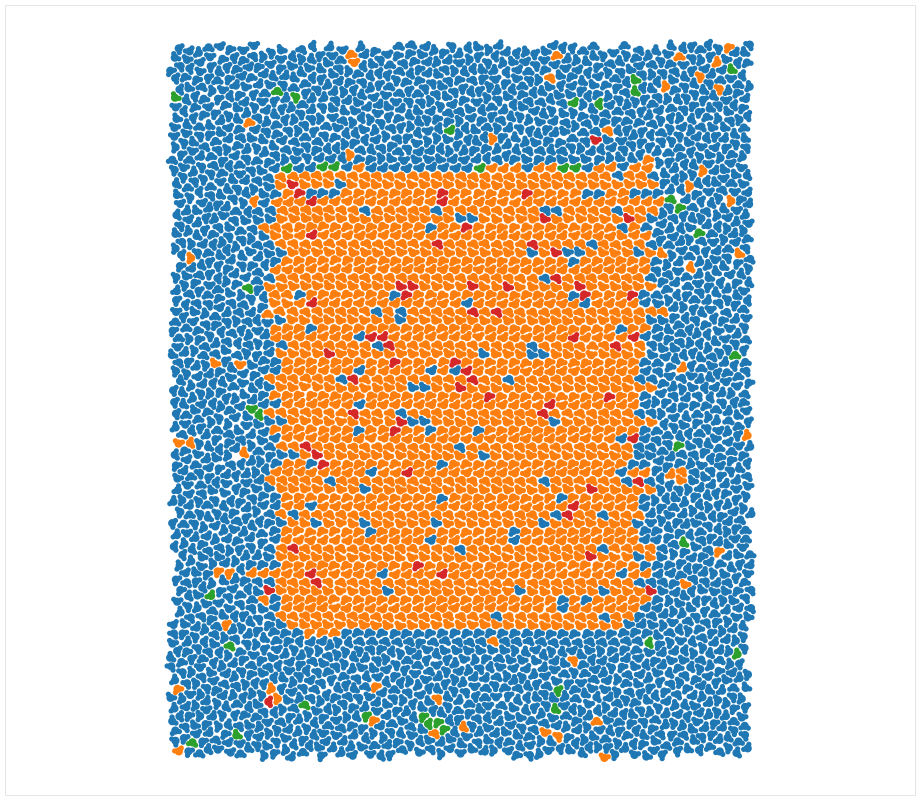
\includegraphics[width=\textwidth]{clustering_results_p2gg.png}
    \end{column}
    \begin{column}{0.33\textwidth}
      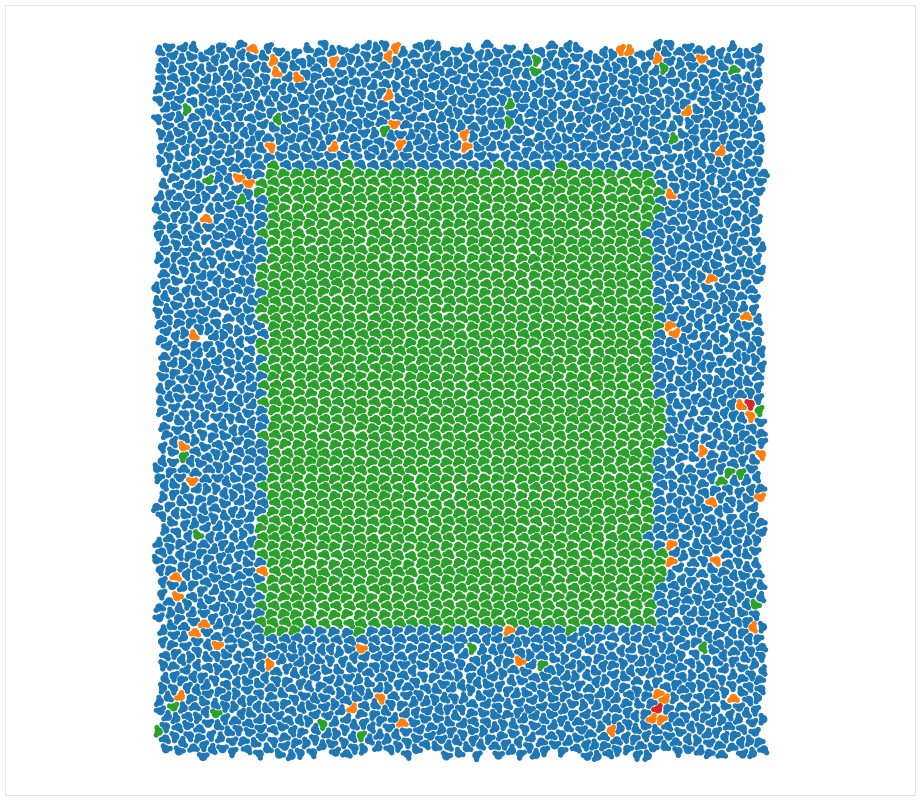
\includegraphics[width=\textwidth]{clustering_results_pg.png}
    \end{column}
  \end{columns}
\end{frame}

\begin{frame}{What now?}

  \begin{itemize}
    \item Clusters are labelled training data
    \item Develop model to apply to a range of structures
  \end{itemize}

\end{frame}


\begin{frame}{Conclusion}

  \begin{itemize}
    \item Features are the most important part of machine learning
    \item Clustering can identify structure within a configuration
    \item Clusters as training data allows for developing a model
  \end{itemize}

\end{frame}


\begin{frame}{How Can I get Involved?}

  \begin{itemize}
    \item Make datasets available (Zenodo or similar)
    \item Check out my project page \url{github.com/malramsay64/MLCrystals}
    \item Try it out yourself
    \item Get in touch \href{mailto:mram5995@uni.sydney.edu.au}{mram5995@uni.sydney.edu.au}
  \end{itemize}

\end{frame}

\end{document}
